\documentclass{beamer}

\usepackage{epsfig}
\usepackage{multicol}
\usepackage{geometry}
%\usepackage[dvipsnames]{xcolor}
\usepackage{textcomp}
\usepackage{graphicx}
\usepackage{caption}
\usepackage{subcaption}
\usepackage{amsmath}
\usepackage{tcolorbox}
\usetheme{Boadilla}
\usepackage{pict2e}
\usepackage{tikz}
\usepackage{xcolor}


\title[Traitement du signal numérique]{Traitement du signal numérique - HEI4 IMS}
\author[Antony Bazir]{}

\setlength{\unitlength}{1cm}

\begin{document}
\section{Signaux Biomédicaux}
\subsection{Types de signaux}
\begin{frame}
\frametitle{Signaux Biomédicaux}
Différents types de signaux biomédicaux: \\
\vspace{0.3cm}
\begin{itemize}
\item<2-> Bioéléctriques
\vspace{0.2cm}
\item<3-> Bioimpédances
\vspace{0.2cm}
\item<4-> Bioacoustiques
\vspace{0.2cm}
\item<5-> Biomagnétiques
\vspace{0.2cm}
\item<6-> Biochimiques
\vspace{0.2cm}
\item<7-> Biooptiques
\end{itemize}
\end{frame}

\begin{frame}
\frametitle{Signaux Bioélectriques}
\textbf{Potentiel électrochimique de membrane}
\begin{columns}
\column{60mm}
 \includegraphics[scale=0.2]{membrane_ions2.png}
 \footnotesize \textit{wikipedia.org}
\column{60mm}
\begin{enumerate}
\item Absorption de nutriments extérieurs
\vspace{0.3cm}
\item Conversion en ions/molécules
\vspace{0.3cm}
\item Potentiel de membrane
\end{enumerate}
\vspace{0.4cm}
\begin{itemize}
\item -80 mV et -40 mV par cellules
\vspace{0.2cm}
\item Utilisé par les cellules nerveuses et musculaires pour leur fonctionnement
\end{itemize}
\end{columns}
\end{frame}

\begin{frame}
\frametitle{Signaux Bioélectriques}
\textbf{Potentiel d'action}
\begin{columns}
\column{60mm}
\includegraphics[scale=0.2]{Potentiel_action.png}
\column{60mm}
Changement de potentiel des cellules suite à une excitation
\begin{enumerate}
\item Dépolarisation
\item Repolarisation
\item Période Réfractaire
\item Repos
\end{enumerate}
\end{columns}
\only<2->{
\begin{block}{}
Comment mesurer le potentiel d'action ?
\end{block}
}
\end{frame}

\begin{frame}
\frametitle{Signaux Bioélectriques}
\begin{columns}
\column{60mm}
\includegraphics[scale=0.2]{galvanic.png}\\
\textit{\footnotesize{Principe d'une cellule galvanique}}\\
\vspace{0.3cm}
\small{En aposant des électrodes sur la peau, on recrée des cellules galvaniques\\
\vspace{0.3cm}
Le corps et ses cellules jouent le rôle de solutions ioniques
}


\column{60mm}
\includegraphics[scale=0.3]{electrodes.png}\\
\textit{\footnotesize{Structures possibles d'électrodes et vues en coupe}}\\
\vspace{0.3cm}
\small{Important : Polarisabilité des électrodes\\

\vspace{0.3cm}
\'Electrode hautement polarisable = inadaptées aux mesures basses fréquences

}

\end{columns}
\end{frame}


\begin{frame}
\frametitle{Bioimpédances}
\textbf{\underline{Impédance}} : Extension de la notion de résistance aux tensions/courants alternatifs 
\begin{columns}
\column{60mm}
\begin{center}
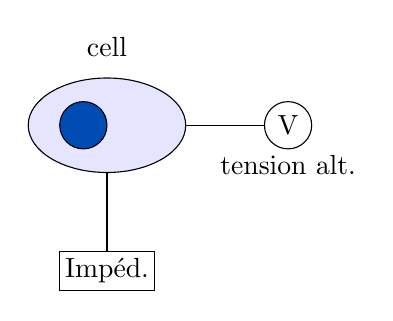
\begin{tikzpicture}
\draw (0,1) node{cell};
\draw[fill=blue!10!white] (0,0) ellipse (1 and 0.6);
\draw[fill=blue!70!green] (-0.3,0) circle(0.3);
\draw(1,0)--(2,0); 
\draw (2.3,0) circle(0.3) node{V};
 \draw (2.3,-0.5) node{tension alt.};
 \draw(0,-0.6)--(0,-1.6); 
 \draw (-0.6,-2.1) rectangle node[text centered]{Impéd.} (0.6,-1.6) ;
\end{tikzpicture} 
\end{center}
\column{60mm}
\begin{itemize}
\item Envoi d'une tension alternative dans le tissu ou la cellule
\vspace{0.2cm}
\item La résistance mesurée informe sur l'état du tissu
\vspace{0.2cm}
\item Fréquence : 50 kHz - 1 MHz 
\vspace{0.2cm}
\item Courant: 2 - 20 mA 
\end{itemize}
\end{columns} 
\end{frame}

\begin{frame}
\frametitle{Bioimpédances}
\textbf{\underline{Impédance}} : Extension de la notion de résistance aux tensions/courants alternatifs 
\begin{columns}
\column{60mm}
\begin{center}
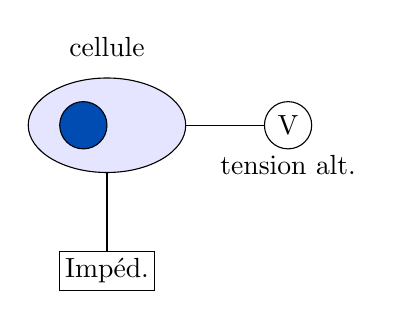
\begin{tikzpicture}
\draw (0,1) node{cellule};
\draw[fill=blue!10!white] (0,0) ellipse (1 and 0.6);
\draw[fill=blue!70!green] (-0.3,0) circle(0.3);
\draw(1,0)--(2,0); 
\draw (2.3,0) circle(0.3) node{V};
 \draw (2.3,-0.5) node{tension alt.};
 \draw(0,-0.6)--(0,-1.6); 
 \draw (-0.6,-2.1) rectangle node[text centered]{Impéd.} (0.6,-1.6) ;
\end{tikzpicture} 
\end{center}
\column{60mm}
\underline{Applications:} 
\begin{itemize}
\item  Suivi respiratoire et détection d'apnée
\vspace{0.4cm}
\item Suivi de flux sanguins dans les membres et détection de thromboses
\vspace{0.4cm}
\item Mesure de composition (taux de tissus adipeux etc...)
\end{itemize}
\end{columns} 
\end{frame}

\begin{frame}
\frametitle{Signaux Bioacoustiques}
\textbf{Ondes mécaniques/acoustiques émises par le corps}
\begin{columns}
\column{60mm}
\begin{center}
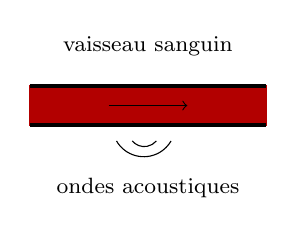
\begin{tikzpicture}
\draw (1.5,1) node[text centered]{\footnotesize vaisseau sanguin};
\draw[red!70!black,fill=red!70!black] (0,0) rectangle (3,0.5);
\draw[ultra thick] (0,0.5)--(3,0.5);
\draw[ultra thick] (0,0)--(3,0);
\draw[->] (1,0.25)--(2,0.25);

\draw (1.3,-0.2)arc (220:320:0.2);
\draw (1.1,-0.2)arc (210:330:0.4);
\draw (1.5,-0.8) node[text centered]{\footnotesize ondes acoustiques};
\end{tikzpicture} 
\end{center}
\textit{Exemple d'ondes acoustiques émises par le corps.}
\column{60mm}
\begin{itemize}
\item Peuvent informer sur la fonction d'un organe
\vspace{0.2cm}
\item Fréquence : 100-1000 Hz 
\vspace{0.2cm}
\item Mesuré par le biais de traducteurs acoustiques
\end{itemize}
\end{columns}
\begin{block}{}
Comment fonctionnent les traducteurs ultrasonores ?
\end{block}
\end{frame}
%https://sigport.org/topic-tags/bioacoustics-and-medical-acoustics pour les exemples

\begin{frame}
\frametitle{Signaux Bioacoustiques}
\textbf{Traducteurs Ultrasonores}
\begin{columns}
\column{70mm}
\includegraphics[scale=0.3]{piezo.png}\\
\textit{\footnotesize{Structure d'un traducteur ultrasonore (J.Bronzino) }}
\column{50mm}
\begin{itemize}
\item Plaque avant (protection)
\vspace{0.2cm}
\item Couche d'adaptation d'impédance 
\vspace{0.2cm}
\item Matériau piézoélectrique
\vspace{0.2cm}
\item Couche arrière 
\end{itemize}
\vspace{0.4cm}
Les traducteurs sont souvent composés de plusieurs éléments
\end{columns}

\end{frame}

\begin{frame}
\frametitle{Signaux Bioacoustiques}
\textbf{Traducteurs Ultrasonores}
\center
\includegraphics[scale=0.4]{phased.png}\\
\textit{\footnotesize{Principe de fonctionnement des traducteurs multiéléments}}

\end{frame}

\begin{frame}
\frametitle{Signaux Biomagnétiques}
\textbf{Courants électriques $\rightarrow$ Champ magnétique}
\begin{columns}
\column{60mm}
\vspace{0.2cm}\\
 \includegraphics[scale=0.3]{biomag_sig.png}\\
 \vspace{0.1cm}
 \textit{B.J. Roth, MDPI, 2023}
\column{60mm}
\begin{itemize}
\item Champs magnétiques faibles 1-100 pT (champ terrestre $\approx$  \textmu T)
\vspace{0.2cm}
\item Fréquence 0.1-1000 Hz
\vspace{0.2cm}
\item Mesuré avec des magnétomètres (bobines)
\vspace{0.2cm}
\item Utile au diagnostic de certaines pathologies neurologiques (epilepsie etc...)
\end{itemize}

\end{columns}
\end{frame}

\begin{frame}
\frametitle{Signaux Biomécaniques}
\textbf{Signaux issus d'actions/contraintes mécaniques liées aux fonctions du corps}
\begin{columns}
\column{60mm}
 \includegraphics[scale=0.33]{gait.png}\\
 \vspace{0.1cm}
 \textit{Mezghani et al., IEEE, 2016}

\column{60mm}
\begin{itemize}
\item Fréquence : 0.001 - 1 Hz
\vspace{0.2cm}
\item Mesures de force, vitesse ou accélération 
\vspace{0.2cm}
\item Pas de propagation $\rightarrow$ mesure potentiellement invasive
\vspace{0.2cm}
\end{itemize}
\end{columns}
\end{frame}

\begin{frame}
\frametitle{Signaux Biomécaniques}
\textbf{Signaux issus d'actions/contraintes mécaniques liées aux fonctions du corps}
\begin{columns}
\column{60mm}
\includegraphics[scale=0.33]{accelerometre.png}\\
\footnotesize{\textit{Schéma de principe d'un accéléromètre (Bronzino)}}
\column{60mm}
\includegraphics[scale=0.33]{mems.png}\\
\footnotesize{\textit{Microaccélèmètre de type MEMS (Bronzino)}}

\end{columns}
\begin{block}{}
Variante non-optique...
\end{block} 

 \end{frame}

\begin{frame}
\frametitle{Signaux Biomécaniques}
\textbf{Signaux issus d'actions/contraintes mécaniques liées aux fonctions du corps}
\begin{columns}
\column{60mm}
\includegraphics[scale=0.23]{lsm6dsm.png}\\
\footnotesize{\textit{Centrale inertielle (STMicroelectronics)}}
\column{60mm}
\includegraphics[scale=0.5]{MotionCapture.jpeg}\\
\footnotesize{\textit{Scène de Motion Capture}}

\end{columns}
\vspace{0.3cm}
\underline{Applications: Biomédical, Navigation, Jeux vidéos, Cinéma...}
\end{frame}

\begin{frame}
\frametitle{Signaux Biochimiques}
\begin{columns}
\column{60mm}
 \includegraphics[scale=0.5]{ABG.png}\\
 \vspace{0.1cm}
 \textit{Cleveland Clinic, 2022}
\column{60mm}
 \underline{Estimation de concentrations}:
\begin{itemize}
\item Marquages immunologiques + fluorescence
\vspace{0.2cm}
\item Mesure photométriques (marqueur + photomètre)
\vspace{0.2cm}
\item Mesure par électrodes
\vspace{0.2cm}
\item Comptage de cellule 
\vspace{0.2cm}
\item Signaux variant généralement très lentement
\end{itemize}
\end{columns}
\end{frame}

\begin{frame}
\frametitle{Signaux Biooptiques}
\textbf{Informations basées sur la détection de lumière ou les propriétés optiques}
\begin{columns}
\column{60mm}
 \includegraphics[scale=0.15]{pox.png}\\
 \vspace{0.1cm}
 \textit{Fonctionnement d'un oxymètre, wikipedia.org}
\column{60mm}
\begin{itemize}
\item Mesures spectrales (différentes longueurs d'onde)
\vspace{0.2cm}
\item Détecter avec des capteurs CMOS ou des photodiodes 
\vspace{0.2cm}
\item Signaux sujets à la diffusion et à la réfraction
\end{itemize}
\end{columns}
\end{frame}

\begin{frame}
\frametitle{Caractéristiques des signaux biomédicaux déterministes}
\begin{center}
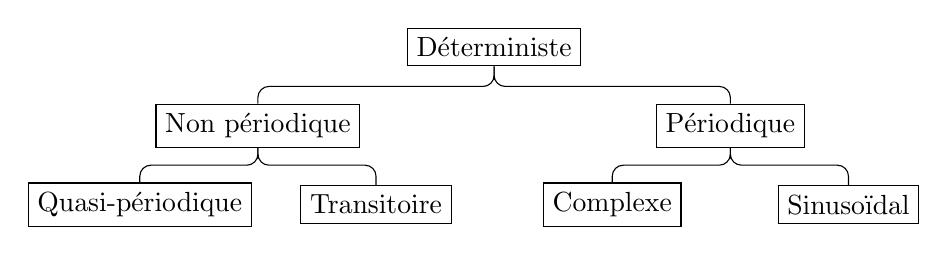
\begin{tikzpicture}
\node[draw,rectangle] (D) at (0,0) {Déterministe};


\node[draw,rectangle] (NP) at (-3,-1) {Non périodique};
\node[draw,rectangle] (P) at (3,-1) {Périodique};
\draw[rounded corners] (D) |- (0,-0.5) -| (NP);
\draw[rounded corners] (D) |- (0,-0.5) -| (P);


\node[draw,rectangle] (S) at (4.5,-2) {Sinusoïdal};
\node[draw,rectangle] (C) at (1.5,-2) {Complexe};
\draw[rounded corners] (P) |- (3,-1.5) -| (S);
\draw[rounded corners] (P) |- (3,-1.5) -| (C);

\node[draw,rectangle] (Q) at (-4.5,-2) {Quasi-périodique};
\node[draw,rectangle] (T) at (-1.5,-2) {Transitoire};
\draw[rounded corners] (NP) |- (-3,-1.5) -| (Q);
\draw[rounded corners] (NP) |- (-3,-1.5) -| (T);
\end{tikzpicture}
\end{center}
\end{frame}

\subsection{Déterministes vs. Stochastiques}
\begin{frame}
\frametitle{Caractéristiques des signaux biomédicaux déterministes}
\textbf{Déterministe }: Peut être prédit et/ou décrit quasi-exactement par une fonction.
\vspace{0.1cm}
\begin{itemize}
\item \textbf{Périodique} 
\vspace{0.1cm}
\begin{itemize}
 \item \textbf{Sinusoïdal:} Pure sinusoïde d'une fréquence et d'une phase donnée
 \vspace{0.1cm}
 \item \textbf{Complexe:} Combinaison d'au moins deux sinusoïdes pures 
\end{itemize}
 \vspace{0.2cm}
\item \textbf{Non-Périodique }
\begin{itemize}
 \vspace{0.1cm}
 \item \textbf{Quasi-Périodique}
 \vspace{0.1cm}
 \item \textbf{Transitoire} 
\end{itemize}
\end{itemize}
\end{frame}

\begin{frame}
\frametitle{Signaux Déterministes Périodiques}
\begin{columns}
\column{60mm}
\underline{\textbf{Sinusoïdal}}: \\
ex: $g_1(t) = 0.55\cos(2 t)$
\begin{center}
\begin{tikzpicture}
\begin{scope}[scale=0.45]
	\draw[->] (-6.28,0)-- (6.28,0);
%\draw (-0.3,-0.3) node {0};
\draw[->] (0,-3)-- (0,3);
\draw (2*pi+0.2,0.25) node {\scriptsize  $t$};
\draw (0,3.5) node {\scriptsize $ g_1(t)$};
%\draw (4.5,-0.3) node {1};

		\draw[domain=-6.28:6.28,color=blue,samples=160] plot (\x,{2*(0.55*cos(2*\x r))});
	\end{scope}
\end{tikzpicture}
\end{center}
\column{60mm}
\underline{\textbf{Complexe}}:\\
ex: $g_2(t) = 0.55\cos(2 t) + 0.45 \cos(4 t + \frac{\pi}{3})$
\begin{center}
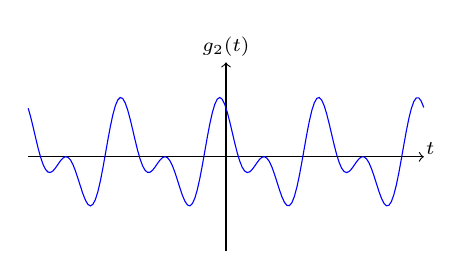
\begin{tikzpicture}
\begin{scope}[scale=0.4,yshift=-6cm]
	\draw[->] (-6.28,0)-- (6.28,0);
%\draw (-0.3,-0.3) node {0};
\draw[->] (0,-3)-- (0,3);
\draw (2*pi+0.2,0.25) node {\scriptsize $t$};
\draw (0,3.5) node {\scriptsize $g_2(t)$};
%\draw (4.5,-0.3) node {1};

		\draw[domain=-6.28:6.28,color=blue,samples=160] plot (\x,{2*(0.55*cos(2*\x r)+ 0.45*cos(2*2*(\x+3.14/12) r))});
	\end{scope}
	\end{tikzpicture}
\end{center}
\end{columns}
\end{frame}

\begin{frame}
\frametitle{Signaux Déterministes Périodiques}
\begin{columns}
\column{60mm}
\underline{\textbf{Quasi-périodique}}: \\
ex: $g_1(t) = \sin(x) + \sin(\pi x)$
\begin{center}
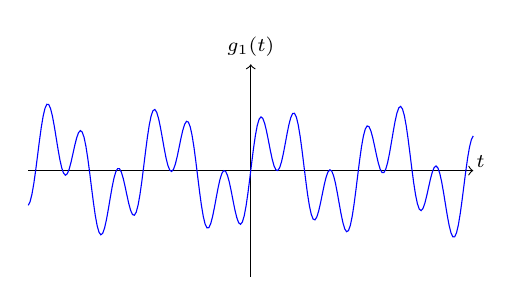
\begin{tikzpicture}
\begin{scope}[scale=0.45]
	\draw[->] (-6.28,0)-- (6.28,0);
%\draw (-0.3,-0.3) node {0};
\draw[->] (0,-3)-- (0,3);
\draw (2*pi+0.2,0.25) node {\scriptsize  $t$};
\draw (0,3.5) node {\scriptsize $ g_1(t)$};
%\draw (4.5,-0.3) node {1};

		\draw[domain=-6.28:6.28,color=blue,samples=240] plot (\x,{1*(sin(2*\x r)+sin(2*3.14*\x r))});
	\end{scope}
\end{tikzpicture}
\end{center}
\column{60mm}
\underline{\textbf{Transitoire}}:\\
ex: $g_2(t) = 1-\exp(-t)$
\begin{center}
\begin{tikzpicture}
\begin{scope}[scale=0.4,yshift=-6cm]
	\draw[->] (-6.28,0)-- (6.28,0);
%\draw (-0.3,-0.3) node {0};
\draw[->] (0,-3)-- (0,3);
\draw (2*pi+0.2,0.25) node {\scriptsize $t$};
\draw (0,3.5) node {\scriptsize $g_2(t)$};
%\draw (4.5,-0.3) node {1};

		\draw[domain=-0:6.28,color=blue,samples=160] plot (\x,{2*(1-exp(-\x))});
	\end{scope}
	\end{tikzpicture}
\end{center}
\end{columns}
\end{frame}


\begin{frame}
\frametitle{Caractéristiques des signaux biomédicaux stochastiques}
\begin{center}
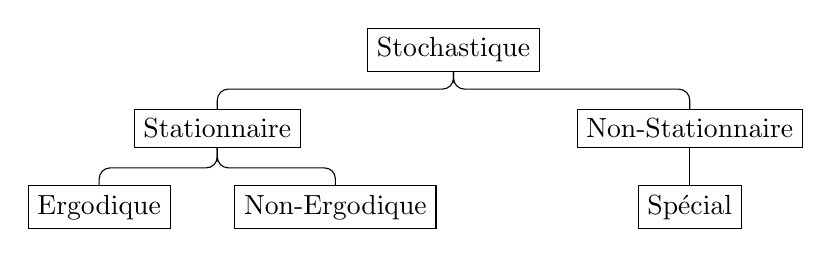
\begin{tikzpicture}

\node[draw,rectangle] (S) at (0,0) {Stochastique};

\node[draw,rectangle] (ST) at (-3,-1) {Stationnaire};
\node[draw,rectangle] (NS) at (3,-1) {Non-Stationnaire};
\draw[rounded corners] (S) |- (0,-0.5) -| (ST);
\draw[rounded corners] (S) |- (0,-0.5) -| (NS);


\node[draw,rectangle] (E) at (-4.5,-2) {Ergodique};
\node[draw,rectangle] (NE) at (-1.5,-2) {Non-Ergodique};
\draw[rounded corners] (ST) |- (-3,-1.5) -| (E);
\draw[rounded corners] (ST) |- (-3,-1.5) -| (NE);

\node[draw,rectangle] (SP) at (3,-2) {Spécial};
\draw[rounded corners] (NS) |- (3,-1.5) -| (SP);

\end{tikzpicture}
\end{center}
\end{frame}

\begin{frame}
\frametitle{Caractéristiques des signaux biomédicaux stochastiques}
\textbf{Stochastique} :  \'Evolution, discrète ou à temps continu, d'une variable aléatoire décrite par des variables statistiques
\vspace{0.2cm}
\begin{itemize}
\item \textbf{Stationnaire:} Les variables statistiques (moyenne variance etc...) sont constantes au cours du temps 
\vspace{0.1cm}
\begin{itemize}
 \item \textbf{Ergodique}:  processus stochastique pour lequel les statistiques peuvent être approchées par l'étude d'une seule réalisation suffisamment longue. 
 \vspace{0.1cm}
 \item \textbf{Non-Ergodique}
\end{itemize}
\vspace{0.2cm}
\item \textbf{Non-Stationnaire}
\vspace{0.1cm}
\begin{itemize}
 \item \textbf{Spécial}
\end{itemize}
\end{itemize}
\end{frame}

\subsection{Exemples de signaux}
\subsubsection{\'Electrocardiogramme}
\begin{frame}
\frametitle{Exemple de signaux : \'Electrocardiogramme (ECG) }
\begin{columns}
\column{60mm}
\includegraphics[scale=0.4]{heart.png}\\
\textit{\footnotesize Schéma du coeur avec ses pacemakers naturels, Najarian \& Splinter}
\column{60mm}
\begin{itemize}
\item Les noeuds "activent" les cellules cardiaques
\vspace{0.5cm}
\item Le changement de potentiel sur l'ensemble de cellules se propage. 
\vspace{0.3cm}
\item On mesure ce potentiel en différents points du corps à la surface de la peau 
\end{itemize}
\end{columns}
\end{frame}

\begin{frame}
\frametitle{Exemple de signaux : \'Electrocardiogramme (ECG)}
\begin{center}
\includegraphics[scale=0.35]{PQRSTU.png}\\
\textit{\footnotesize (a) Forme caractéristique d'un ECG. (b) ECG d'un patient normal. Najarian \& Splinter}
\end{center}
\begin{itemize}
\item Le signal correspond aux polarisations/dépolarisations de différentes parties du coeur.
\item Chaque partie du signal a une durée de $\approx$ 100 ms
\item Chaque partie contient de l'information qui doit potentiellement être analysée.
\end{itemize}
\end{frame}

\begin{frame}
\frametitle{Exemple de signaux : \'Electrocardiogramme (ECG)}
\begin{center}
\includegraphics[scale=0.35]{PQRSTU.png}\\
\textit{\footnotesize (a) Forme caractéristique d'un ECG. (b) ECG d'un patient normal. Najarian \& Splinter}
\end{center}
De plus, le contenu fréquentiel des parties peut évoluer en fonction de l'état du patient
\vspace{0.1cm}
\begin{block}{}
Comment analyser ces signaux  ?
\end{block}
\end{frame}

\begin{frame}
\frametitle{Exemple de signaux : \'Electrocardiogramme (ECG)}
\begin{center}
\includegraphics[scale=0.32]{PQRSTU.png}\\
\textit{\footnotesize (a) Forme caractéristique d'un ECG. (b) ECG d'un patient normal. Najarian \& Splinter}
\end{center}
Dans ce cas, la transformée de Fourier est peu utile...
\begin{itemize}
\item Transformée de Fourier court terme/Short-term Fourier Transform (STFT)
\item Analyse en ondelettes
\item Algorithmes spécifiques
\end{itemize}
\end{frame}

\begin{frame}
\frametitle{Analyse de signaux}
\textbf{Transformée de Fourier court terme/Short-term Fourier Transform (STFT)}
\vspace{1cm}
\begin{columns}
\column{60mm}
\underline{Produit de convolution}:
$(f \star g) (x) =  \displaystyle \int^{\infty}_{-\infty} f(x-t)g(t) \; dt  $
\column{60mm}
\underline{Transformée de Fourier}:
	$ TF\{ f \}(\nu) = \displaystyle \int^{\infty}_{-\infty} f(t) e^{-j2\pi \nu t} dt $
\end{columns}
\vspace{1cm}
TFCT/STFT: TF du produit d'un \textbf{signal} $f(t)$ et d'une \textbf{fenêtre} $w(t)$ centrée sur $\tau$.\\

\[ \boxed{STFT\{ f \}(\tau,\nu) =  \int^{\infty}_{-\infty} w(t-\tau )f(t) e^{-j2\pi \nu t }\; dt} \] 

\end{frame}

%\begin{frame}
%\frametitle{Analyse ECG STFT}
%
%	\begin{center}
%	\begin{tikzpicture}
%	\begin{scope}[scale=1]
%\draw[->] (0,0)-- (7,0)node[right] {\scriptsize $t$} ;
%\draw (6,-0.3)node {\scriptsize $6$} ;
%\draw (0,-0.3)node {\scriptsize $0$} ;
%\draw[->] (0,0)-- (0,4)node[above] {\scriptsize  $e(t)$};
%\draw[thick,blue] plot file {ecg_1.txt};
%	\end{scope}
%	\end{tikzpicture}
%	\end{center}
%	\footnotesize{\textit{Signal d'ECG}}
%
%\end{frame}

\begin{frame}
\frametitle{Analyse en Ondelettes}
La transformée de Fourier 'projète' le signal sur une base de sinusoïde...\\
\vspace{0.5cm}
\only<2->{
Pas toujours adaptée...\\
\vspace{0.5cm}
}
\only<3->{
\textbf{"Continuous Wavelet Transform"/"Transformée en ondelettes continue"}
\[ \boxed{CWT\{s(t) \}(a,b) = \frac{1}{\sqrt{a}}\int^{\infty}_{-\infty}s(t)\overline{\phi}(\frac{t-b}{a})\; dt} \]
}
\only<4->{
\begin{itemize}
\item $s(t)$ : signal à analyser
\item $\phi(t)$ : ondelette d'analyse
\item $a$ : facteur d'élargissement/contraction
\item $b$ : décalage temporel
\end{itemize}
}
\end{frame}

\begin{frame}
\frametitle{Analyse en Ondelettes}
La transformée de Fourier 'projète' le signal sur une base de sinusoïde...\\
\vspace{0.5cm}


Pas toujours adaptée...\\
\vspace{0.5cm}

\textbf{"Continuous Wavelet Transform"/"Transformée en ondelettes continue"}
\[ \boxed{CWT\{s(t) \}(a,b) = \frac{1}{\sqrt{a}}\int^{\infty}_{-\infty}s(t)\overline{\phi}(\frac{t-b}{a})\; dt} \]
\vspace{0.5cm}
\only<2>{
\begin{block}{}
Convolution entre l'ondelette et le signal $\longrightarrow$ Localisation de l'énergie dans le signal
\end{block}
}
\end{frame}

\begin{frame}
\frametitle{Analyse en Ondelettes: exemple}
\textbf{Effet d'une angioplastie sur un ECG}\\
\vspace{0.3cm}
%\includegraphics[scale=0.25]{ecg_2.png}\\
%\textit{\footnotesize ECG avant angioplastie, Gramatikov 1995 }
\begin{columns}
\column{60mm}
\includegraphics[scale=0.27]{coarse_wavelet.png}
\column{60mm}
\includegraphics[scale=0.27]{details_ecg.png}
\end{columns}
\textit{\footnotesize Deux familles d'ondelettes utilisées pour la transformée multirésolution, Gramatikov 1995 }
\end{frame}

\begin{frame}
\frametitle{Analyse en Ondelettes: exemple}
\textbf{Effet d'une angioplastie sur un ECG}\\
\vspace{0.3cm}
%\includegraphics[scale=0.25]{ecg_2.png}\\
%\textit{\footnotesize ECG avant angioplastie, Gramatikov 1995 }
\begin{columns}
\column{60mm}
\includegraphics[scale=0.27]{coarse_wavelet.png}
\column{60mm}
Remarques: 
\begin{itemize}
\item Chaque fonction correspond à une étape de décomposition
\item \`A chaque étape on divise la fréquence d'échantillonnage par deux
\end{itemize}
\end{columns}
\end{frame}

\begin{frame}
\frametitle{Analyse en Ondelettes: exemple}
\textbf{Effet d'une angioplastie sur un ECG}\\
\vspace{0.3cm}
%\includegraphics[scale=0.25]{ecg_2.png}\\
%\textit{\footnotesize ECG avant angioplastie, Gramatikov 1995 }
\begin{columns}
\column{60mm}
\includegraphics[scale=0.30]{scaling.jpg}\\
\includegraphics[scale=0.30]{wavelet.png}\\

\column{60mm}
\includegraphics[scale=0.36]{ecg_decomp.png}

\end{columns}
\textit{\footnotesize Construction des signaux "détails" et "approximation", Gramatikov 1995 }
\end{frame}

\begin{frame}
\frametitle{Analyse en Ondelettes: exemple}
\textbf{Effet d'une angioplastie sur un ECG}\\
\vspace{0.3cm}
%\includegraphics[scale=0.25]{ecg_2.png}\\
%\textit{\footnotesize ECG avant angioplastie, Gramatikov 1995 }
\begin{columns}
\column{60mm}
\includegraphics[scale=0.30]{ecg_3.png}\\


\column{60mm}
\includegraphics[scale=0.36]{results_decomp.png}\\

\end{columns}
\textit{\footnotesize Résultats de la méthode multirésolution, Gramatikov 1995 }\\
\vspace{0.3cm}
\only<2->{
\begin{block}{}
Le changement peut être quantifié par la décomposition
\end{block}
}
\end{frame}

\begin{frame}
\frametitle{Exemple de signaux : \'Electrocardiogramme (ECG)}
\begin{center}
\includegraphics[scale=0.3]{chaine_ECG.png}\\
\textit{\footnotesize Exemple chaîne de traitement d'un ECG Tompkins, 2000}
\end{center}
\begin{enumerate}
\item 1ère étape de filtrage analogique
\item Conversion en numérique en vue d'analyse et de post-traitement
\end{enumerate}
\end{frame}

\begin{frame}
\frametitle{Exemple de signaux : \'Electrocardiogramme (ECG)}
\begin{center}
\includegraphics[scale=0.35]{tr_num_ecg.png}\\
\textit{\footnotesize Algorithme de détection du complexe QRS, Tompkins, 2000}\\
\end{center}
Filtrage temps réel du signal numérique \& Extraction du QRS
\begin{enumerate}
\item<2-> filtrage passe-bande pour ne garder que les fréquences du QRS
\item<3-> Dérivée du signal (QRS = forte pente)
\item<4-> Mise au carré (signal positif et haute fréquences accentuées)
\item<5-> Moyennage
\end{enumerate}
\only<6->{On reviendra sur cette chaine de traitement plus en détail...}
\end{frame}

\subsubsection{\'Electroencéphalogramme}
\begin{frame}
\frametitle{Exemple de signaux : \'Electroencéphalogramme (EEG)}
\begin{center}
\includegraphics[scale=0.35]{EEG_electrodes.png}\\
\textit{\footnotesize Placement des électrodes pour un EEG. Najarian \& Splinter}
\end{center}
\vspace{0.2cm}
\begin{itemize}
\item Amplification des signaux de polarisation/dépolarisation des cellules nerveuses
\item On mesure généralement des potentiels évoqués par des stimuli
\end{itemize}

\end{frame}

\begin{frame}
\frametitle{Exemple de signaux : \'Electroencéphalogramme (EEG)}
\begin{columns}
\column{60mm}
\includegraphics[scale=0.33]{EEG.png}\\
\textit{\footnotesize Signaux EEG. Najarian \& Splinter}
\column{60mm}
\begin{itemize}
\item Signaux stochastiques 
\vspace{0.2cm}
\item Analyse spectral : Détection des ondes $\alpha$, $\beta$, $\delta$ et $\theta$
\vspace{0.2cm}
\item Analyse dans le domaine temporel pour les potentiels évoqués
\end{itemize}
\end{columns}
\end{frame}

\begin{frame}
\frametitle{Exemple de signaux : \'Electroencéphalogramme (EEG)}
\begin{columns}
\column{60mm}
\includegraphics[scale=0.33]{evp_eeg.png}\\
\textit{\footnotesize Signaux EEG avec stimuli. Najarian \& Splinter}
\column{60mm}
Dans ce cas, on va vouloir détecter le signal dans le domaine temporel
\end{columns}

\end{frame}

\begin{frame}
\frametitle{Exemple de signaux : \'Electroencéphalogramme (EEG)}
\begin{columns}
\column{60mm}
\includegraphics[scale=0.3]{evp_moy.png}\\
\textit{\footnotesize Moyennage d'un EEG avec stimuli. Bronzino, 2010}
\column{60mm}
\begin{itemize}
\item Signal brut très bruité $\rightarrow$ stimuli difficilement identifiable
\vspace{0.2cm}
\item Le bruit est de nature stochastique 
\vspace{0.2cm}
\item Le signal se reproduit environ toujours au même temps
\vspace{0.2cm}
\item Le moyennage amplifie le signal et élimine le bruit.
\end{itemize}
\end{columns}

\end{frame}

\subsubsection{Ultrasons}
\begin{frame}
\frametitle{Exemple de signaux : Ultrasons}
\begin{columns}
\column{60mm}
\includegraphics[scale=0.23]{Ultrasonic.png}\\
\textit{\footnotesize Principe d'imagerie ultrasonore. Hazari, 2010}
\column{60mm}
\begin{enumerate}
\item<2-> \textbf{\'Emission} ultrasonore vers la zone d'intérêt
\vspace{0.2cm}
\item<3-> \textbf{Détection} du signal ultrasonore transmis, réfléchi ou diffusé
\vspace{0.2cm}
\item<4-> \textbf{Traitement/Analyse} du signal reçu
\end{enumerate}
\end{columns}
\end{frame}


\begin{frame}
\frametitle{Exemple de signaux : Ultrasons}
\begin{columns}
\column{60mm}
\includegraphics[scale=0.23]{A-scan.png}\\
\textit{\footnotesize A-scan en imagerie ultrasonore. Hazari, 2010}
\column{60mm}
Pour un traducteur unique:
\vspace{0.2cm}
\begin{enumerate}
\item<2-> \'Emission du signal par excitation électrique
\vspace{0.2cm}
\item<3-> Propagation et réflexions aux interfaces 
\vspace{0.2cm}
\item<4-> Réception par le traducteur
\end{enumerate}
\vspace{0.2cm}
\only<4->{\textbf{Unité de base de l'imagerie ultrasonore}}
\end{columns}
\end{frame}

\begin{frame}
\frametitle{Exemple de signaux : Ultrasons}
\begin{center}
\includegraphics[scale=0.25]{B-scan.png}\\
\textit{\footnotesize B-scans en imagerie ultrasonore. Hazari, 2010}\\
\end{center}
On dispose généralement d'un réseau de traducteurs qui vont former les pixels de l'image\\
\vspace{0.2cm}
\begin{enumerate}
\item<2-> \textbf{Conversion} des A-scans en niveau de gris
\vspace{0.2cm}
\item<3-> \textbf{Cartographie spatiale} des signaux résultants 
\end{enumerate}
\vspace{0.2cm}

\end{frame}

\begin{frame}
\frametitle{Exemple de signaux : Ultrasons}
\textbf{Chaine de traitement pour les signaux ultrasonores}\\
\begin{center}
\includegraphics[scale=0.33]{chaine_us.png}\\
\textit{\footnotesize Chaîne de traitement en imagerie ultrasonore. Hazari, 2010}\\
\end{center}
\begin{itemize}
\item<2-> Premier filtrage analogique 
\item<3-> Conversion en numérique
\item<4-> Traitements mathématiques numériques 
\end{itemize}
\end{frame}

\begin{frame}
\frametitle{Exemple de signaux : Ultrasons}
\begin{columns}
\column{60mm}
\includegraphics[scale=0.23]{Ultrasonic.png}\\
\textit{\footnotesize Principe d'imagerie ultrasonore. Hazari, 2010}
\column{60mm}
Applications:
\begin{itemize}
\item Imagerie de contraste $\rightarrow$ variation \textbf{relative} prop. méca\\
\begin{itemize}
\item Détection de discontinuité/interfaces 
\end{itemize}
\vspace{0.2cm}
\item Mesure \textbf{absolue} prop. méca 
\begin{itemize}
\item Mesure pulse-écho  
\item Mesure régime sinusoïdal
\end{itemize}
\vspace{0.2cm}
\item \textbf{Cartographie} propriétés mécaniques
\begin{itemize}
\item carte vitesse du son 
\item carte atténuation
\end{itemize}
\end{itemize}
\end{columns}
\end{frame}

\subsubsection{Rayons-X/$\gamma$}
\begin{frame}
\frametitle{Exemple de signaux : Rayons-X/$\gamma$}
Principe :
\[  I = I_0 \cdot \exp (- \int^{x_{max}}_{x_0} \; \mu (Z(x),E) \; dx)  \] 
\vspace{0.5cm}
\begin{itemize}
\item $I_0, I$: intensités initiale et détectée 
\item $x_0, x_{max}$ : Points d'entrée et de sortie de l'objet à imager
\item $Z(x)$  numéro atomique du matériau traversé 
\item $E$ énergie du rayonnement émis
\end{itemize}
\vspace{0.5cm}
\only<2->{
\textbf{Offre un contraste entre différents tissus}
}
\end{frame}

\begin{frame}
\frametitle{Exemple de signaux : Rayons-X/$\gamma$}
\begin{columns}
\column{60mm}
\begin{center}
\includegraphics[scale=0.12]{xray_plan.jpg}\\
\textit{Radiographie pulmonaire numérisée, Nevit Delmen}
\end{center}
\column{60mm}
\begin{center}
\includegraphics[scale=0.22]{xray_tomo.png}\\
\textit{Tomographie axiale calculée, Mustafa Mafraji}
\end{center}
\end{columns}
\end{frame}

\begin{frame}
\frametitle{Exemple de signaux : Rayons-X/$\gamma$}
\begin{center}
\includegraphics[scale=0.3]{dig_mammo.png}\\
\end{center}
\begin{itemize}
\item Radiographie numérique : Comptage de photons/mesure d'énergie $\rightarrow$ signal numérique
\item Standard actuel dans le domaine médical
\item Outils de traitement d'image numérique disponible
\end{itemize}
\end{frame}

\begin{frame}
\frametitle{Exemple de signaux: résumé}
\begin{itemize}
\item \textbf{\'Electrocardiogramme }
\begin{itemize}
\item signal bioélectrique
\item Analyse fréquentielle 
\item Détection de motifs (QRS, RR, etc...)
\end{itemize}
\vspace{0.1cm}
\item \textbf{\'Electroencéphalogramme}
\begin{itemize}
\item signal bioélectrique
\item Analyse fréquentielle (ondes $\alpha$, $\beta$, $\delta$...) 
\item Détection de motifs (ondes évoquées)
\end{itemize}
\vspace{0.1cm}
\item  \textbf{Ultrasons} 
\begin{itemize}
\item signal acoustique
\item mesure des propriétés acoustiques  (rigidité, etc...)
\item imagerie de contraste (échographie, tomographie, etc...)
\end{itemize}
\vspace{0.1cm}
\item \textbf{Rayons-X/$\gamma$}
\begin{itemize}
\item signal electromagnétique
\item imagerie de contraste (échographie, tomographie, etc...)
\end{itemize}
\end{itemize} 
\end{frame}

\subsection{Chaîne d'instrumentation Numérique}
\begin{frame}
\frametitle{Chaine d'instrumentation Numérique}
\begin{center}
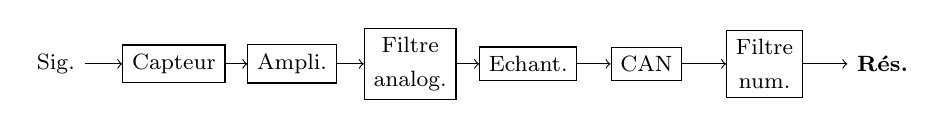
\begin{tikzpicture}
\node (S) at (0,0) {\footnotesize  Sig.};
\node[draw,rectangle,align=center]  (C) at (1.5,0) {\footnotesize Capteur}; 
\node[draw,rectangle,align=center]  (A) at (3,0) {\footnotesize Ampli.}; 
\node[draw,rectangle,align=center]  (F) at (4.5,0) {\footnotesize Filtre \\ \footnotesize analog.}; 
\node[draw,rectangle,align=center]  (E) at (6,0) {\footnotesize Echant.}; 
\node[draw,rectangle,align=center]  (AD) at (7.5,0) {\footnotesize CAN}; 
\node[draw,rectangle,align=center]  (N) at (9,0) {\footnotesize Filtre \\ \footnotesize num.}; 
\node (R) at (10.5,0) {\footnotesize  \textbf{Rés.}};

\draw[->] (S)--(C);
\draw[->] (C)--(A);
\draw[->] (A)--(F);
\draw[->] (F)--(E);
\draw[->] (E)--(AD);
\draw[->] (AD)--(N);
\draw[->] (N)--(R);
\end{tikzpicture}
\end{center}
\begin{enumerate}
\item Conversion du signal physique en tension
\item Amplification
\item Filtrage analogique
\item \'Echantillonnage  (Bloqueur)
\item Conversion analogique-numérique
\item Filtrage numérique 
\end{enumerate}
\vspace{0.3cm}
\only<2->{
Des variantes existent...
}
\end{frame}

\begin{frame}
\frametitle{Chaine d'instrumentation Numérique : Capteur}
\begin{center}
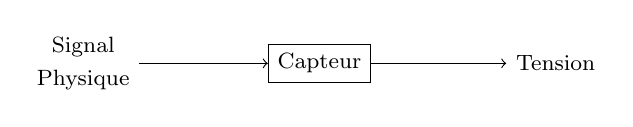
\begin{tikzpicture}
\node[align=center] (S) at (0,0) {\footnotesize  Signal\\ \footnotesize  Physique};
\node[draw,rectangle,align=center]  (C) at (3,0) {\footnotesize Capteur};
\node[align=center] (T) at (6,0) {\footnotesize  Tension};

\draw[->] (S)--(C);
\draw[->] (C)--(T);
\end{tikzpicture}
\end{center}
\vspace{0.1cm}
\textbf{Caractéristiques :}\\
\vspace{0.1cm}
\begin{itemize}
\item Conversion \textbf{univoque} entre le signal physique et la tension
\vspace{0.1cm}
\item Gamme de mesure et/ou Plage de linéarite
\vspace{0.1cm}
\item \textbf{Résolution} spatiale et temporelle
\vspace{0.1cm}
\item Exemples : 
\begin{itemize}
\item Tradcuteur piézoélectrique
\vspace{0.1cm}
\item Détecteur à comptage de photons
\vspace{0.1cm}
\item Electrodes ECG/EEG
\end{itemize}
\vspace{0.1cm}
\end{itemize}
\end{frame}

\begin{frame}
\frametitle{Chaine d'instrumentation Numérique : Amplificateur}
\begin{center}
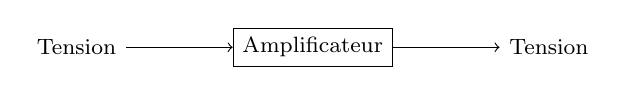
\begin{tikzpicture}
\node[align=center] (S) at (0,0) {\footnotesize  Tension};
\node[draw,rectangle,align=center]  (C) at (3,0) {\footnotesize Amplificateur};
\node[align=center] (T) at (6,0) {\footnotesize  Tension};

\draw[->] (S)--(C);
\draw[->] (C)--(T);
\end{tikzpicture}
\end{center}
\vspace{0.1cm}
\textbf{Caractéristiques :}\\
\vspace{0.1cm}
\begin{itemize}
\item \textbf{Applique un facteur multplicatif sur le signal du capteur}
\vspace{0.1cm}
\item Adapte la tension à la gamme de CAN
\vspace{0.1cm}
\item Doit être \textbf{linéaire en tension ET en fréquence}
\vspace{0.1cm}
\item Amplifie également le bruit 
\vspace{0.1cm}
\begin{itemize}
\item nécessité potentielle d'un premier filtrage 
\vspace{0.1cm}
\item  filtre notch 50 Hz...
\end{itemize}
\end{itemize}
\end{frame}

\begin{frame}
\frametitle{Chaine d'instrumentation Numérique : Filtrage analogique}
\begin{center}
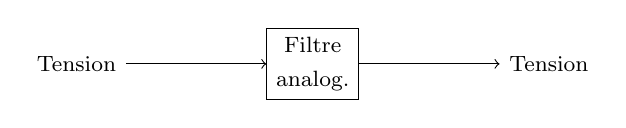
\begin{tikzpicture}
\node[align=center] (S) at (0,0) {\footnotesize  Tension};
\node[draw,rectangle,align=center]  (C) at (3,0) {\footnotesize Filtre \\ \footnotesize analog.};
\node[align=center] (T) at (6,0) {\footnotesize  Tension};

\draw[->] (S)--(C);
\draw[->] (C)--(T);
\end{tikzpicture}
\end{center}
\vspace{0.1cm}
\textbf{Caractéristiques :}\\
\vspace{0.2cm}
\begin{itemize}
\item \textbf{Souvent utilisé pour éliminer des parasites bien identifiés }
\vspace{0.2cm}
\begin{itemize}
\item Passe-bas : Bruit des électrodes (EEG/ECG)
\vspace{0.2cm}
\item Notch : élimination du 50-60 Hz
\vspace{0.2cm}
\item Passe-haut : élimination de la respiration/mouvments corporels (ultrasons)
\end{itemize}
\end{itemize}
\end{frame}

\begin{frame}
\frametitle{Chaine d'instrumentation Numérique : \'Echantillonnage}
\begin{center}
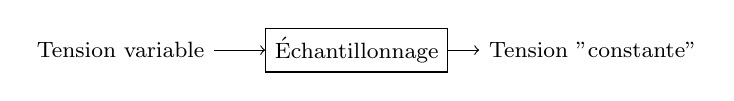
\begin{tikzpicture}
\node[align=center] (S) at (0,0) {\footnotesize  Tension variable};
\node[draw,rectangle,align=center]  (C) at (3,0) {\footnotesize \'Echantillonnage};
\node[align=center] (T) at (6,0) {\footnotesize  Tension "constante"};

\draw[->] (S)--(C);
\draw[->] (C)--(T);
\end{tikzpicture}
\end{center}
\vspace{0.1cm}
\textbf{\textbf{Circuit bloqueur} :}\\
\vspace{0.2cm}
\begin{itemize}
\item \textbf{Prend la valeur en  entrée et la maintient pendant $T_e$ }
\vspace{0.2cm}
\begin{itemize}
\item Retard d'ouverture 
\vspace{0.2cm}
\item Incertitude d'ouverture 
\vspace{0.2cm}
\item Temps d'établissement du blocage
\end{itemize}
\vspace{0.2cm}
\item Temps caractéristiques \textbf{bien inférieurs} à la période d'échantillonnage.
\end{itemize}
\end{frame}

\begin{frame}
\frametitle{Chaine d'instrumentation Numérique : Conversion Analogique/Numérique}
\begin{center}
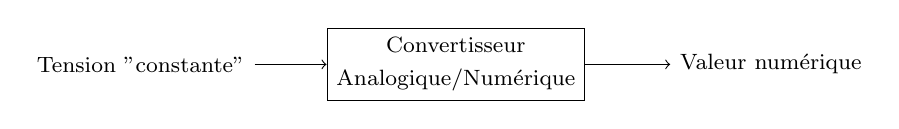
\begin{tikzpicture}
\node[align=center] (S) at (0,0) {\footnotesize  Tension "constante"};
\node[draw,rectangle,align=center]  (C) at (4,0) {\footnotesize Convertisseur \\ \footnotesize  Analogique/Numérique};
\node[align=center] (T) at (8,0) {\footnotesize  Valeur numérique};

\draw[->] (S)--(C);
\draw[->] (C)--(T);
\end{tikzpicture}
\end{center}
\vspace{0.1cm}
\begin{itemize}
\item \textbf{Convertit la valeur réelle en valeur binaire}
\vspace{0.2cm}
\begin{itemize}
\item Gamme dynamique divisé en N échelons  
\vspace{0.2cm}
\item Valeur réelle située dans un échelon pendant $T_e$
\vspace{0.2cm}
\item Correspondance à une valeur numérique (001 , 010, 00011..)
\end{itemize}
\vspace{0.2cm}
\item Plusieurs architectures possibles (Double rampe, Sigma-delta...) basées sur des cycles de charge-décharges suivies dans le temps
\end{itemize}
\end{frame}

\begin{frame}
\frametitle{Chaine d'instrumentation Numérique : Filtrage numérique}
\begin{center}
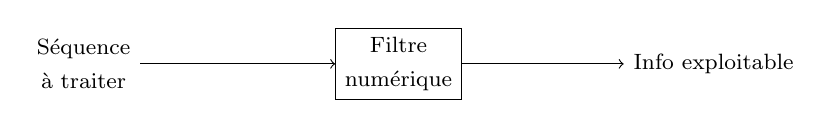
\begin{tikzpicture}
\node[align=center] (S) at (0,0) {\footnotesize  Séquence \\
\footnotesize à traiter};
\node[draw,rectangle,align=center]  (C) at (4,0) {\footnotesize Filtre \\ \footnotesize  numérique};
\node[align=center] (T) at (8,0) {\footnotesize  Info exploitable};

\draw[->] (S)--(C);
\draw[->] (C)--(T);
\end{tikzpicture}
\end{center}
\vspace{0.1cm}
\begin{itemize}
\item \textbf{Extraction ou réorganisation de l'info}
\vspace{0.2cm}
\begin{itemize}
\item A-scan $\rightarrow$ Image complète (ultrasons) 
\vspace{0.2cm}
\item Plans de projection $\rightarrow$ Vue en coupe (radiographie)
\vspace{0.2cm}
\item Signaux temporels $\rightarrow$ variables pertinentes (ECG, EEG, etc...)
\end{itemize}
\vspace{0.2cm}
\end{itemize}
\end{frame}

\begin{frame}
\frametitle{Chaine d'instrumentation Numérique}
\begin{center}
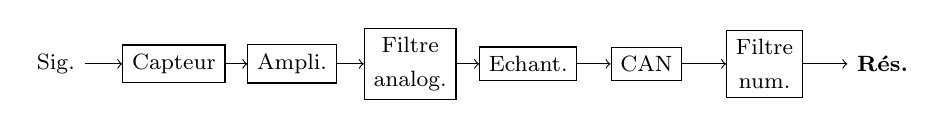
\begin{tikzpicture}
\node (S) at (0,0) {\footnotesize  Sig.};
\node[draw,rectangle,align=center]  (C) at (1.5,0) {\footnotesize Capteur}; 
\node[draw,rectangle,align=center]  (A) at (3,0) {\footnotesize Ampli.}; 
\node[draw,rectangle,align=center]  (F) at (4.5,0) {\footnotesize Filtre \\ \footnotesize analog.}; 
\node[draw,rectangle,align=center]  (E) at (6,0) {\footnotesize Echant.}; 
\node[draw,rectangle,align=center]  (AD) at (7.5,0) {\footnotesize CAN}; 
\node[draw,rectangle,align=center]  (N) at (9,0) {\footnotesize Filtre \\ \footnotesize num.}; 
\node (R) at (10.5,0) {\footnotesize  \textbf{Rés.}};

\draw[->] (S)--(C);
\draw[->] (C)--(A);
\draw[->] (A)--(F);
\draw[->] (F)--(E);
\draw[->] (E)--(AD);
\draw[->] (AD)--(N);
\draw[->] (N)--(R);
\end{tikzpicture}
\end{center}
\begin{enumerate}
\item Conversion du signal physique en tension
\item Amplification
\item Filtrage analogique
\item \'Echantillonnage  (Bloqueur)
\item Conversion analogique-numérique
\item \textbf{Filtrage numérique} 
\end{enumerate}
\vspace{0.3cm}
\only<2->{
On va se concentrer sur la partie filtrage... numérique
}
\end{frame}

  
\end{document}
